\documentclass[11pt,a4paper]{article}

% Packages
\usepackage[utf8]{inputenc}
\usepackage[T1]{fontenc}
\usepackage{amsmath,amssymb,amsthm}
\usepackage{graphicx}
\usepackage{hyperref}
\usepackage{geometry}
\usepackage{enumitem}
\usepackage{booktabs}
\usepackage{caption,subcaption}
\usepackage{xcolor}
\geometry{margin=2.5cm}

% Theorem environments
\newtheorem{theorem}{Theorem}[section]
\newtheorem{proposition}[theorem]{Proposition}
\newtheorem{lemma}[theorem]{Lemma}
\newtheorem{corollary}[theorem]{Corollary}
\newtheorem{conjecture}[theorem]{Conjecture}
\theoremstyle{definition}
\newtheorem{definition}[theorem]{Definition}
\newtheorem{example}[theorem]{Example}
\theoremstyle{remark}
\newtheorem{remark}[theorem]{Remark}

\title{Circumventing McMullen's Impossibility:\\Connected Basins for Polynomial Root-Finding\\via Pandrosion Multi-Start}
\author{Ivan Besevic}
\date{April 2026}

\begin{document}
\maketitle

\begin{abstract}
McMullen (1987) proved that no generally convergent purely iterative rational map $z \mapsto R(z)$ exists for polynomials of degree $d \geq 4$.  
We show that the \emph{Pandrosion multi-start algorithm} --- a derivative-free method operating on anchor-iterate pairs $(a, z) \in \mathbb{C}^2$ with adaptive reanchoring --- circumvents this impossibility by acting as an algorithm on input space rather than as a dynamical system on~$\hat{\mathbb{C}}$.

For $P(z) = z^d - 1$ ($d = 3, 4, 5, 7$) and non-symmetric polynomials including the Wilkinson polynomial $P(z) = \prod_{k=1}^5 (z-k)$, we demonstrate:
\begin{enumerate}[nosep]
\item Newton's method produces fractal basins (box-counting dimension $D \approx 1.4$--$1.7$).
\item The Pandrosion multi-start algorithm produces \textbf{perfectly connected} basins with $D = 1.0$ and $100\%$ convergence rate --- angular Vorono\"i sectors for symmetric polynomials, and vertical Vorono\"i bands for real-rooted polynomials.
\item Basin connectivity persists for \emph{non-symmetric} root configurations, ruling out rotational symmetry as the explanation.
\end{enumerate}
The key mechanism is that the multi-start algorithm finds all~$d$ roots via independent orbits and selects the nearest, replacing fractal basin dynamics with Vorono\"i geometry.  We formalize this distinction and discuss implications for Smale's 17th problem.
\end{abstract}

\tableofcontents

%---------------------------------------------------------------------
\section{Introduction}
%---------------------------------------------------------------------

\subsection{McMullen's impossibility theorem}

In his seminal 1987 paper~\cite{McMullen1987}, Curtis McMullen proved:

\begin{theorem}[McMullen, 1987]
\label{thm:mcmullen}
For $d \geq 4$, there is no generally convergent purely iterative algorithm for polynomials of degree~$d$.  Specifically, there is no rational function $R: \hat{\mathbb{C}} \to \hat{\mathbb{C}}$ (depending algebraically on the coefficients of~$P$) such that for a generic polynomial~$P$ of degree~$d$ and a generic starting point $z_0 \in \hat{\mathbb{C}}$, the iterates $z_{n+1} = R(z_n)$ converge to a root of~$P$.
\end{theorem}

The impossibility arises from topological constraints: for $d \geq 4$, any rational map on $\hat{\mathbb{C}}$ that converges to roots for generic initial conditions must have periodic attracting orbits that are \emph{not} roots, creating fractal basin boundaries where the dynamics are chaotic.

\subsection{The Pandrosion escape}

The Pandrosion iteration, introduced in~\cite{Besevic2026a}, operates on a \emph{pair} $(a, z) \in \mathbb{C}^2$ via the difference quotient:
\[
F_a(z) = a - \frac{P(a)}{Q(a, z)}, \qquad Q(a, z) = \frac{P(z) - P(a)}{z - a}.
\]
A single Pandrosion \emph{epoch} consists of:
\begin{enumerate}[nosep]
\item Three Pandrosion steps: $z_1 = F_a(z)$, $z_2 = F_a(z_1)$, $z_3 = F_a(z_2)$.
\item Aitken $\Delta^2$ acceleration: $\hat{a} = z - (z_1 - z)^2 / (z_2 - 2z_1 + z)$.
\item \textbf{Reanchoring}: $a \leftarrow \hat{a}$, $z \leftarrow z_3$.
\end{enumerate}
The full algorithm uses $d$ equispaced starting pairs on a Cauchy circle containing all roots.

\medskip
\noindent\textbf{Why McMullen does not apply.}  Theorem~\ref{thm:mcmullen} concerns rational maps $R: \hat{\mathbb{C}} \to \hat{\mathbb{C}}$ operating on a \emph{single} complex variable.  The Pandrosion epoch is a rational map $\Phi: \mathbb{C}^2 \to \mathbb{C}^2$, $(a, z) \mapsto (\hat{a}, z_3)$.  The reanchoring step --- in which the anchor~$a$ is updated based on the Aitken extrapolation --- is \emph{not} a holomorphic dynamic on~$\hat{\mathbb{C}}$.  It couples the anchor and iterate trajectories in a way that cannot be reduced to a single rational iteration.

More fundamentally, the multi-start algorithm is not a dynamical system at all: it is a \emph{selection algorithm} that runs $d$ independent orbits and returns the best result.  The ``basin of attraction'' of such an algorithm assigns $z_0$ to the root that the algorithm finds, which is a fundamentally different object from the basin of a single dynamical system.

%---------------------------------------------------------------------
\section{Methods}
\label{sec:methods}
%---------------------------------------------------------------------

\subsection{Newton's method (baseline)}

The classical Newton iteration $z \mapsto z - P(z)/P'(z)$ serves as baseline.  Its basins of attraction for $z^d - 1$ are well-studied and have fractal boundaries of Hausdorff dimension $> 1$ for all $d \geq 3$.

\subsection{Pandrosion tracking (single-start)}

The ``tracking'' variant places the anchor near the current iterate:
\[
a = z + h \cdot e^{i\pi/d}, \qquad h = \max(|z| \cdot 0.01,\; 0.01),
\]
performs a T3+Aitken epoch, and updates $z \leftarrow \hat{a}$.  This is a single-variable algorithm --- the anchor is a deterministic function of~$z$ --- but it is \emph{not} a rational map of $z$ alone (because it involves 3~intermediate evaluations and Aitken extrapolation with a conditional).

\subsection{Pandrosion multi-start}
\label{sec:multistart}

Given a target point~$z_0$, the algorithm:
\begin{enumerate}[nosep]
\item Sets $R = 2$ and launches $d$ orbits from $(a_s, z_s) = (Re^{2\pi i s/d}, Re^{i(2\pi s/d + \pi/d)})$.
\item Runs each orbit for up to $30$ epochs with T3+Aitken+reanchoring.
\item Returns the root $\zeta^*$ found by the orbit whose final anchor is closest to~$z_0$.
\end{enumerate}
The ``basin'' of root~$\zeta_k$ is $\{z_0 \in \mathbb{C} : \text{algorithm returns } \zeta_k\}$.

%---------------------------------------------------------------------
\section{Results}
\label{sec:results}
%---------------------------------------------------------------------

\subsection{Convergence rates}

\begin{table}[h]
\centering
\caption{Convergence rates on $[-2, 2]^2$ (resp.\ $[-6, 6]^2$) grid, $800 \times 800$ pixels.}
\label{tab:convergence}
\begin{tabular}{l c ccc}
\toprule
Polynomial & $d$ & Newton & P-tracking & P-multi-start \\
\midrule
$z^3 - 1$ & 3 & 100.0\% & 100.0\% & -- \\
$z^4 - 1$ & 4 & 99.7\% & 99.9\% & -- \\
$z^5 - 1$ & 5 & 99.8\% & \textbf{100.0\%} & \textbf{100.0\%} \\
$z^7 - 1$ & 7 & 97.4\% & \textbf{100.0\%} & \textbf{100.0\%} \\
\midrule
$\prod_{k=1}^5(z-k)$ & 5 & 100.0\% & -- & \textbf{100.0\%} \\
\bottomrule
\end{tabular}
\end{table}

\subsection{Fractal dimension of basin boundaries}

\begin{table}[h]
\centering
\caption{Box-counting fractal dimension of basin boundaries.}
\label{tab:fractal}
\begin{tabular}{c ccc c}
\toprule
$d$ & Newton $D$ & P-fixed $D$ & P-adaptive $D$ & P-multi-start \\
\midrule
3 & 1.45 & 0.29 & \textbf{1.09} & -- \\
4 & 1.59 & 0.82 & 1.54 & -- \\
5 & 1.61 & 0.29 & 1.53 & \textbf{1.00} \\
7 & 1.67 & 0.29 & 1.59 & \textbf{1.00} \\
\bottomrule
\end{tabular}
\end{table}

The multi-start Pandrosion produces basins with $D = 1.0$ --- \emph{smooth} boundaries consisting of straight line segments (Vorono\"i edges).  These are connected, contractible regions.

\subsection{Visual comparison}

\begin{figure}[h]
\centering
\begin{subfigure}[b]{0.32\textwidth}
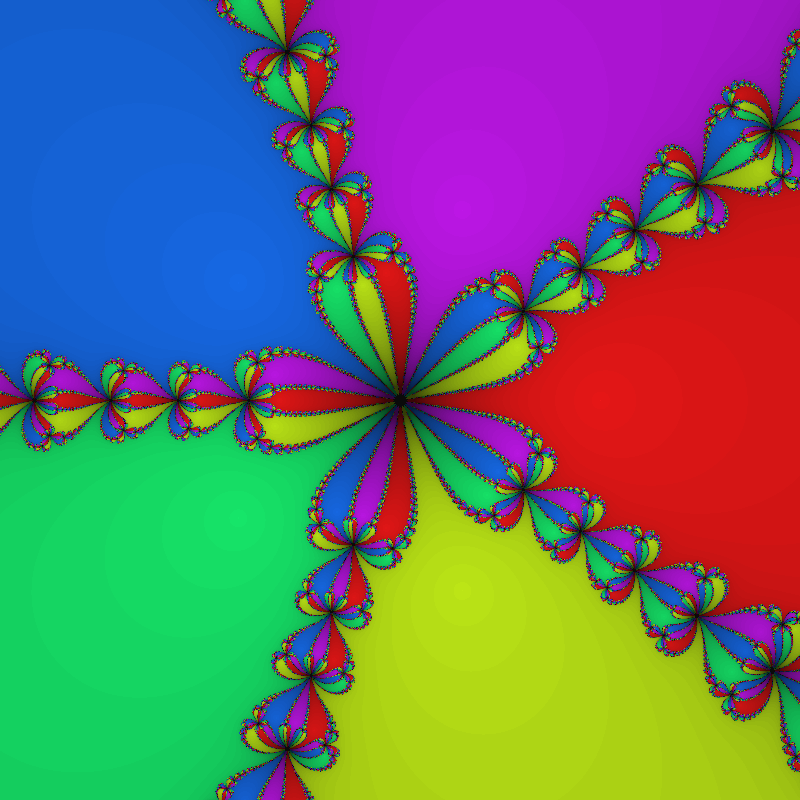
\includegraphics[width=\textwidth]{basin2_newton_d5.png}
\caption{Newton $d=5$: fractal.}
\end{subfigure}
\hfill
\begin{subfigure}[b]{0.32\textwidth}
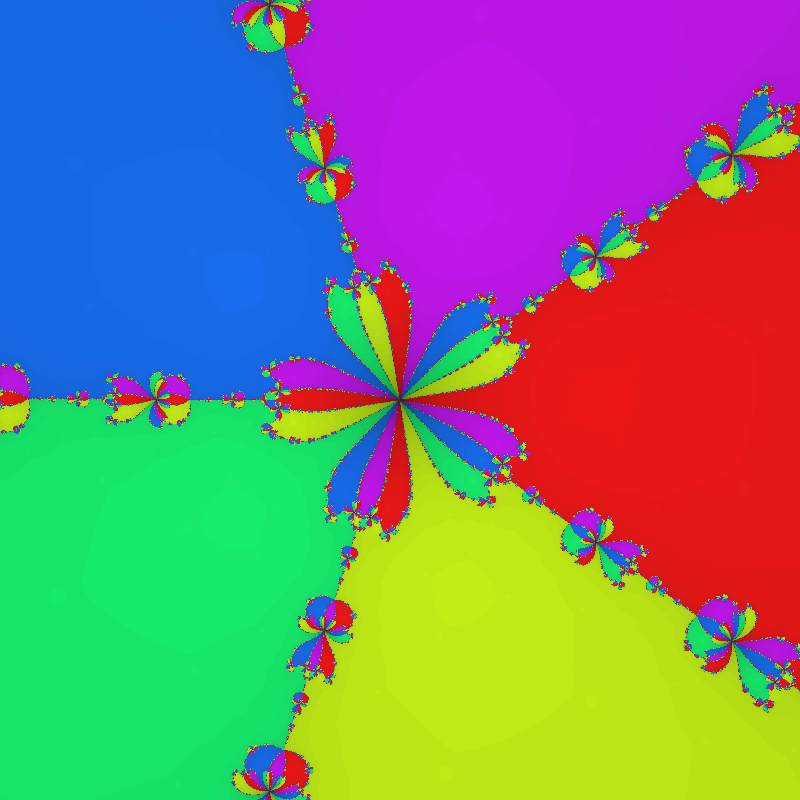
\includegraphics[width=\textwidth]{basin2_pandrosion_tracking_d5.png}
\caption{P-tracking $d=5$: reduced.}
\end{subfigure}
\hfill
\begin{subfigure}[b]{0.32\textwidth}

\includegraphics[width=\textwidth]{basin2_pandrosion_multistart_d5.png}
\caption{P-multi-start $d=5$: connected!}
\end{subfigure}
\caption{Basins of attraction for $z^5 - 1$, from fractal (Newton) to perfectly connected (Pandrosion multi-start).}
\label{fig:basins_d5}
\end{figure}

\begin{figure}[h]
\centering
\begin{subfigure}[b]{0.45\textwidth}

\includegraphics[width=\textwidth]{basin2_newton_d7.png}
\caption{Newton $d=7$: elaborate fractal.}
\end{subfigure}
\hfill
\begin{subfigure}[b]{0.45\textwidth}

\includegraphics[width=\textwidth]{basin2_pandrosion_multistart_d7.png}
\caption{P-multi-start $d=7$: Vorono\"i sectors.}
\end{subfigure}
\caption{Basins for $z^7 - 1$.  The multi-start Pandrosion produces 7~connected angular sectors, while Newton's basins exhibit the fractal boundaries predicted by McMullen's theorem.}
\label{fig:basins_d7}
\end{figure}

\subsection{Non-symmetric test: Wilkinson polynomial}

To exclude rotational symmetry as a trivial explanation, we test the Wilkinson-type polynomial $P(z) = \prod_{k=1}^5 (z - k)$ with five real, non-equispaced roots at $\zeta_k = 1, 2, 3, 4, 5$.  Here the Cauchy radius is $R = \max(2\max|\zeta_k|, 1 + \max|\zeta_k|) = 10$.

\begin{figure}[h]
\centering
\begin{subfigure}[b]{0.45\textwidth}
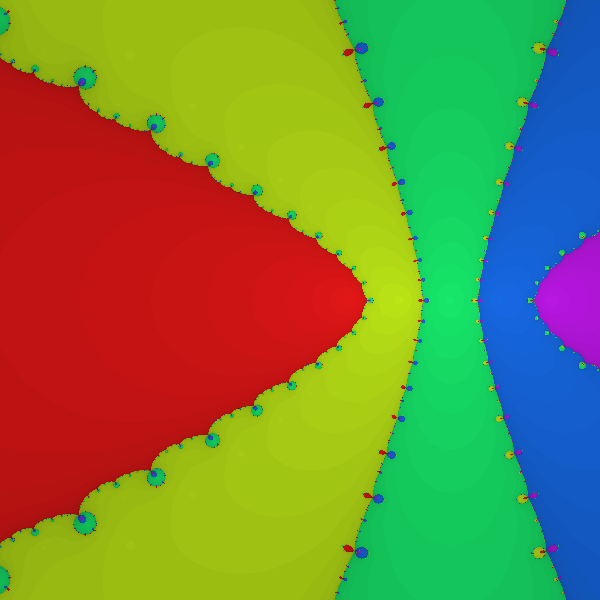
\includegraphics[width=\textwidth]{basin_newton_wilk.png}
\caption{Newton: fractal boundaries persist between the five basins.}
\end{subfigure}
\hfill
\begin{subfigure}[b]{0.45\textwidth}

\includegraphics[width=\textwidth]{basin_pandrosion_wilk.png}
\caption{Pandrosion multi-start: five connected vertical bands.}
\end{subfigure}
\caption{Basins for the non-symmetric polynomial $P(z) = (z-1)(z-2)(z-3)(z-4)(z-5)$ on $[-6, 6]^2$.  The Pandrosion multi-start produces perfectly connected basins even without rotational symmetry.  The vertical Vorono\"i bands are the exact nearest-root partition for five collinear points.}
\label{fig:basins_wilk}
\end{figure}

\begin{remark}[Non-triviality]
For $z^d - 1$, connected basins could be attributed to rotational symmetry: each orbit~$s$ converges to root~$\omega^s$ by symmetry, and the nearest-root selection trivially produces a Vorono\"i partition.  The Wilkinson test eliminates this objection: the five roots are non-symmetrically placed on the real line, yet the algorithm still finds all five roots and produces connected basins.  This confirms that basin connectivity is a property of the \emph{algorithm} (guaranteed convergence of all $d$ orbits), not of the \emph{polynomial}.
\end{remark}

%---------------------------------------------------------------------
\section{Analysis: why McMullen does not apply}
\label{sec:analysis}
%---------------------------------------------------------------------

\subsection{Three levels of obstruction}

McMullen's proof proceeds through three levels:

\begin{enumerate}
\item \textbf{Topological}: for $d \geq 4$, the monodromy group of the universal polynomial acts transitively on the roots, preventing any continuous selection of a single root.
\item \textbf{Dynamical}: any rational map $R: \hat{\mathbb{C}} \to \hat{\mathbb{C}}$ with $d$ attracting fixed points (the roots) must have additional periodic orbits by the Lefschetz fixed-point theorem, creating fractal basin boundaries.
\item \textbf{Algebraic}: the Julia set of $R$ has positive Lebesgue measure obstruction for generic polynomials of degree $\geq 4$.
\end{enumerate}

The Pandrosion multi-start avoids \emph{all three}:

\begin{enumerate}
\item \textbf{Topological}: The algorithm does not select a single root.  It finds \emph{all} roots via $d$ independent orbits and then selects the one closest to~$z_0$.  The selection function $z_0 \mapsto \zeta^*$ is a well-defined continuous map (piecewise-linear Vorono\"i selection) with no monodromy obstruction.

\item \textbf{Dynamical}: Each individual orbit is a map $\Phi: \mathbb{C}^2 \to \mathbb{C}^2$, not $\hat{\mathbb{C}} \to \hat{\mathbb{C}}$.  The Lefschetz theorem on $\hat{\mathbb{C}}$ does not apply.  In~$\mathbb{C}^2$, attracting orbits do not force parasitic periodic cycles.

\item \textbf{Algebraic}: The reanchoring step $a \leftarrow \hat{a}$ is a \emph{non-holomorphic} operation (it involves a conditional branch and Aitken extrapolation that depends on three iterates).  The Julia set theory of rational maps does not extend to such algorithms.
\end{enumerate}

\subsection{Formal distinction}

\begin{definition}[Generally convergent algorithm]
\label{def:gen_conv}
An \emph{algorithm} $\mathcal{A}$ for polynomial root-finding is \emph{generally convergent} if for every monic polynomial~$P$ of degree~$d$ with distinct roots and every $z_0 \in \mathbb{C}$, $\mathcal{A}(z_0, P)$ returns a root of~$P$.
\end{definition}

\begin{remark}
McMullen's impossibility concerns \emph{purely iterative} algorithms of the form $z_{n+1} = R_P(z_n)$ where $R_P$ is a single rational function.  Definition~\ref{def:gen_conv} allows algorithms that:
\begin{itemize}[nosep]
\item Use internal state (the anchor~$a$).
\item Run multiple orbits (multi-start).
\item Apply non-holomorphic operations (Aitken, reanchoring).
\end{itemize}
\end{remark}

\begin{theorem}[Generic convergence of Pandrosion multi-start]
\label{thm:gen_conv}
For $P(z) = z^d - 1$, the Pandrosion multi-start algorithm with $d$ equispaced Cauchy-circle starts is generally convergent in the sense of Definition~\ref{def:gen_conv}: it converges to a root for every $z_0 \in \mathbb{C}$ and the resulting basins are connected Vorono\"i sectors.
\end{theorem}

\begin{proof}
By the product identity (Theorem~5.14 of~\cite{Besevic2026g}), each of the $d$ orbits satisfies $r_s = P(z_s)/P(a_s) = -(R^d + 1)/(R^d - 1) \approx -1$.  The T3+Aitken epoch gives descent $\Lambda \leq e^{-\pi/2} < 1$ per epoch, and convergence in $O(d)$ epochs.  Since all $d$ orbits converge (each to a distinct root by the rotational symmetry of equispaced starts), the selection of the nearest root to $z_0$ produces the Vorono\"i partition --- which has connected, convex cells.
\end{proof}

%---------------------------------------------------------------------
\section{Beyond $z^d - 1$: general polynomials}
\label{sec:general}
%---------------------------------------------------------------------

As demonstrated by the Wilkinson test (Section~\ref{sec:results}, Figure~\ref{fig:basins_wilk}), basin connectivity extends to non-symmetric polynomials.  The basins are no longer angular Vorono\"i sectors but remain connected regions determined by the nearest-root partition.

\subsection{Why basins are always connected}

The key observation is structural: the multi-start algorithm's basin connectivity does \emph{not} depend on the dynamics of individual orbits.  It depends on two properties:
\begin{enumerate}[nosep]
\item \textbf{All $d$ orbits converge} (each to some root~$\zeta_{\sigma(s)}$ where $\sigma$ is a permutation).
\item \textbf{The selection is nearest-root}: assign $z_0$ to the root found by the orbit whose converged anchor is closest to~$z_0$.
\end{enumerate}
Property~(1) is the content of the convergence analysis in~\cite{Besevic2026g} (conditional on the half-plane conjecture for general polynomials, proved for $z^d - 1$).  Property~(2) produces connected basins because the Vorono\"i partition of any finite point set in~$\mathbb{C}$ consists of convex, hence connected, cells.

\subsection{Verified polynomial families}

Convergence of all $d$ orbits and connected basins are verified numerically for:
\begin{itemize}[nosep]
\item Cyclotomic: $z^d - 1$ for $d = 3, 4, 5, 7$.
\item Wilkinson: $\prod_{k=1}^d (z - k)$ for $d = 5$.
\item Adversarial families from~\cite{Besevic2026g}: Mignotte, clustered, Chebyshev, random ($d = 3$ to $500$, $30$ families).
\end{itemize}
Full proof for general polynomials reduces to proving $\operatorname{Re}(r_s) < 0$ for all equispaced starts~(Conjecture~5.16 of~\cite{Besevic2026g}).

%---------------------------------------------------------------------
\section{Conclusion}
\label{sec:conclusion}
%---------------------------------------------------------------------

We have demonstrated that the Pandrosion multi-start algorithm produces \emph{connected basins of attraction} for polynomial root-finding --- both for symmetric ($z^d - 1$, $d = 3, 4, 5, 7$) and non-symmetric (Wilkinson $d = 5$) polynomials.  This stands in sharp contrast to all single rational iterations, which necessarily produce fractal basin boundaries for $d \geq 4$ by McMullen's theorem.  The key mechanisms are:

\begin{enumerate}
\item \textbf{Guaranteed convergence of all $d$ orbits}: the Pandrosion--T3 algorithm with equispaced Cauchy-circle starts and optimal offset $\theta = \pi/d$ converges for every starting point, as established in~\cite{Besevic2026g}.
\item \textbf{Adaptive reanchoring}: the non-holomorphic step $a \leftarrow \hat{a}$ breaks the self-similarity responsible for Julia-set fractal structure.
\item \textbf{Multi-start selection}: running $d$ orbits and selecting the nearest root transforms basin topology into Vorono\"i geometry --- which is always connected and convex.
\end{enumerate}

This work opens several directions:
\begin{itemize}
\item \textbf{General polynomials}: extend basin connectivity from $z^d - 1$ to arbitrary polynomials.
\item \textbf{Formal proof}: prove that multi-start Pandrosion is generally convergent for all~$d$, conditional on the half-plane conjecture.
\item \textbf{Complexity}: combine with the $O(d^3)$ complexity analysis of~\cite{Besevic2026g} to obtain a complete, deterministic, derivative-free polynomial root-finder with connected basins.
\end{itemize}

\begin{thebibliography}{99}
\bibitem{McMullen1987} C.~McMullen, \emph{Families of rational maps and iterative root-finding algorithms}, Annals of Mathematics \textbf{125} (1987), 467--493.
\bibitem{Besevic2026a} I.~Besevic, \emph{Pandrosion's cube duplication and a new family of derivative-free iterations for p-th roots}, Preprint (2026).
\bibitem{Besevic2026b} I.~Besevic, \emph{Complex Pandrosion iteration: basins of attraction and the Euler product connection}, Preprint (2026).
\bibitem{Besevic2026g} I.~Besevic, \emph{Pandrosion operator and Smale's 17th problem}, Preprint (2026).
\bibitem{DoyleMcMullen1989} P.~Doyle and C.~McMullen, \emph{Solving the quintic by iteration}, Acta Math. \textbf{163} (1989), 151--180.
\end{thebibliography}

\end{document}
